\documentclass[preprint]{elsarticle}

\usepackage{multirow}
\usepackage{lineno}
\usepackage{xspace}
\usepackage{threeparttable}
\usepackage{caption}
\usepackage{subcaption}
\modulolinenumbers[5]

%% Journal name here
\journal{EPJ N}

%% `Elsevier LaTeX' style
\bibliographystyle{elsarticle-num}
%%%%%%%%%%%%%%%%%%%%%%%

%%%% packages and definitions (optional)
\usepackage{placeins}
\usepackage{booktabs} % nice rules (thick lines) for tables
\usepackage{microtype} % improves typography for PDF
\usepackage{hhline}
\usepackage{amsmath}

\usepackage{threeparttable, tablefootnote}

\usepackage{tabularx}

%% Special typesetting for Cyclus
\newcommand{\Cyclus}{\textsc{Cyclus}\xspace}%
\newcommand{\Cycamore}{\textsc{Cycamore}\xspace}%
\graphicspath{{images/}}

% tikz %
\usepackage{tikz}
\usetikzlibrary{shapes.geometric, arrows}
\usetikzlibrary{positioning, arrows, decorations, shapes}

\tikzstyle{facility} = [rectangle, rounded corners, minimum width=2cm, minimum height=0.75cm,text centered, draw=black, fill=blue!30]
\tikzstyle{transition} = [rectangle, rounded corners, minimum width=2cm, minimum height=0.75cm,text centered, draw=black, fill=red!30]
\tikzstyle{arrow} = [thick,->,>=stealth]

% hyperref %
\usepackage[hidelinks]{hyperref}
% after hyperref %
\usepackage{cleveref}
\usepackage{datatool}
\usepackage[acronym,toc]{glossaries}
\newacronym[longplural={metric tons of heavy metal}]{MTHM}{MTHM}{metric ton of heavy metal}
\newacronym{ABM}{ABM}{agent-based modeling}
\newacronym{ACDIS}{ACDIS}{Program in Arms Control \& Domestic and International Security}
\newacronym{AHTR}{AHTR}{Advanced High Temperature Reactor}
\newacronym{ANDRA}{ANDRA}{Agence Nationale pour la gestion des D\'echets RAdioactifs, the French National Agency for Radioactive Waste Management}
\newacronym{APP}{APP}{Abbott Power Plant}
\newacronym{ANL}{ANL}{Argonne National Laboratory}
\newacronym{API}{API}{application programming interface}
\newacronym{ARCH}{ARCH}{autoregressive conditional heteroskedastic}
\newacronym{ARE}{ARE}{Aircraft Reactor Experiment}
\newacronym{ARFC}{ARFC}{Advanced Reactors and Fuel Cycles}
\newacronym{ARMA}{ARMA}{autoregressive moving average}
\newacronym{ASME}{ASME}{American Society of Mechanical Engineers}
\newacronym{ATWS}{ATWS}{Anticipated Transient Without Scram}
\newacronym{BDBE}{BDBE}{Beyond Design Basis Event}
\newacronym{BIDS}{BIDS}{Berkeley Institute for Data Science}
\newacronym{BOL}{BOL}{Beginning-of-Life}
\newacronym{BSD}{BSD}{Berkeley Software Distribution}
\newacronym{CAFCA}{CAFCA}{ Code for Advanced Fuel Cycles Assessment }
\newacronym{CASL}{CASL}{Consortium for Advanced Simulation of Light Water Reactors}
\newacronym{CDTN}{CDTN}{Centro de Desenvolvimento da Tecnologia Nuclear}
\newacronym{CEA}{CEA}{Commissariat \`a l'\'Energie Atomique et aux \'Energies Alternatives}
\newacronym{CI}{CI}{continuous integration}
\newacronym{CNEC}{CNEC}{Consortium for Nonproliferation Enabling Capabilities}
\newacronym{CNEN}{CNEN}{Comiss\~{a}o Nacional de Energia Nuclear}
\newacronym{CNERG}{CNERG}{Computational Nuclear Engineering Research Group}
\newacronym{COSI}{COSI}{Commelini-Sicard}
\newacronym{COTS}{COTS}{commercial, off-the-shelf}
\newacronym{CSNF}{CSNF}{commercial spent nuclear fuel}
\newacronym{CTAH}{CTAHs}{Coiled Tube Air Heaters}
\newacronym{CUBIT}{CUBIT}{CUBIT Geometry and Mesh Generation Toolkit}
\newacronym{CURIE}{CURIE}{Centralized Used Fuel Resource for Information Exchange}
\newacronym{DAG}{DAG}{directed acyclic graph}
\newacronym{DANESS}{DANESS}{Dynamic Analysis of Nuclear Energy System Strategies}
\newacronym{DBE}{DBE}{Design Basis Event}
\newacronym{DESAE}{DESAE}{Dynamic Analysis of Nuclear Energy Systems Strategies}
\newacronym{DHS}{DHS}{Department of Homeland Security}
\newacronym{DOE}{DOE}{Department of Energy}
\newacronym{DRACS}{DRACS}{Direct Reactor Auxiliary Cooling System}
\newacronym{DRE}{DRE}{dynamic resource exchange}
\newacronym{DSNF}{DSNF}{DOE spent nuclear fuel}
\newacronym{DYMOND}{DYMOND}{Dynamic Model of Nuclear Development }
\newacronym{EBS}{EBS}{Engineered Barrier System}
\newacronym{EDZ}{EDZ}{Excavation Disturbed Zone}
\newacronym{EIA}{EIA}{U.S. Energy Information Administration}
\newacronym{EPA}{EPA}{Environmental Protection Agency}
\newacronym{EP}{EP}{Engineering Physics}
\newacronym{FCO}{FCO}{Fuel Cycle Options}
\newacronym{FCT}{FCT}{Fuel Cycle Technology}
\newacronym{FCWMD}{FCWMD}{Fuel Cycle and Waste Management Division}
\newacronym{FEHM}{FEHM}{Finite Element Heat and Mass Transfer}
\newacronym{FEPs}{FEPs}{Features, Events, and Processes}
\newacronym{FHR}{FHR}{Fluoride-Salt-Cooled High-Temperature Reactor}
\newacronym{FLiBe}{FLiBe}{Fluoride-Lithium-Beryllium}
\newacronym{GCAM}{GCAM}{Global Change Assessment Model}
\newacronym{GDSE}{GDSE}{Generic Disposal System Environment}
\newacronym{GDSM}{GDSM}{Generic Disposal System Model}
\newacronym{GENIUSv1}{GENIUSv1}{Global Evaluation of Nuclear Infrastructure Utilization Scenarios, Version 1}
\newacronym{GENIUSv2}{GENIUSv2}{Global Evaluation of Nuclear Infrastructure Utilization Scenarios, Version 2}
\newacronym{GENIUS}{GENIUS}{Global Evaluation of Nuclear Infrastructure Utilization Scenarios}
\newacronym{GPAM}{GPAM}{Generic Performance Assessment Model}
\newacronym{GRSAC}{GRSAC}{Graphite Reactor Severe Accident Code}
\newacronym{GUI}{GUI}{graphical user interface}
\newacronym{HALEU}{HALEU}{High-Assay Low-Enriched Uranium}
\newacronym{HEU}{HEU}{High-Enriched Uranium}
\newacronym{HLW}{HLW}{high level waste}
\newacronym{HPC}{HPC}{high-performance computing}
\newacronym{HTC}{HTC}{high-throughput computing}
\newacronym{HTGR}{HTGR}{High Temperature Gas-Cooled Reactor}
\newacronym{IAEA}{IAEA}{International Atomic Energy Agency}
\newacronym{IEMA}{IEMA}{Illinois Emergency Mangament Agency}
\newacronym{INL}{INL}{Idaho National Laboratory}
\newacronym{IPRR1}{IRP-R1}{Instituto de Pesquisas Radioativas Reator 1}
\newacronym{IRP}{IRP}{Integrated Research Project}
\newacronym{ISFSI}{ISFSI}{Independent Spent Fuel Storage Installation}
\newacronym{ISRG}{ISRG}{Independent Student Research Group}
\newacronym{JFNK}{JFNK}{Jacobian-Free Newton Krylov}
\newacronym{LANL}{LANL}{Los Alamos National Laboratory}
\newacronym{LBNL}{LBNL}{Lawrence Berkeley National Laboratory}
\newacronym{LCOE}{LCOE}{levelized cost of electricity}
\newacronym{LDRD}{LDRD}{laboratory directed research and development}
\newacronym{LEU}{LEU}{Low-Enriched Uranium}
\newacronym{LFR}{LFR}{Lead-Cooled Fast Reactor}
\newacronym{LGPL}{LGPL}{Lesser GNU Public License}
\newacronym{LLNL}{LLNL}{Lawrence Livermore National Laboratory}
\newacronym{LMFBR}{LMFBR}{Liquid-Metal-cooled Fast Breeder Reactor}
\newacronym{LOFC}{LOFC}{Loss of Forced Cooling}
\newacronym{LOHS}{LOHS}{Loss of Heat Sink}
\newacronym{LOLA}{LOLA}{Loss of Large Area}
\newacronym{LP}{LP}{linear program}
\newacronym{LWR}{LWR}{Light Water Reactor}
\newacronym{MARKAL}{MARKAL}{MARKet and ALlocation}
\newacronym{MA}{MA}{minor actinide}
\newacronym{MCNP}{MCNP}{Monte Carlo N-Particle code}
\newacronym{MILP}{MILP}{mixed-integer linear program}
\newacronym{MIT}{MIT}{the Massachusetts Institute of Technology}
\newacronym{MMR}{MMR}{Micro Modular Reactor}
\newacronym{MOAB}{MOAB}{Mesh-Oriented datABase}
\newacronym{MOOSE}{MOOSE}{Multiphysics Object-Oriented Simulation Environment}
\newacronym{MOX}{MOX}{mixed oxide}
\newacronym{MSBR}{MSBR}{Molten Salt Breeder Reactor}
\newacronym{MSRE}{MSRE}{Molten Salt Reactor Experiment}
\newacronym{MSR}{MSR}{Molten Salt Reactor}
\newacronym{NAGRA}{NAGRA}{National Cooperative for the Disposal of Radioactive Waste}
\newacronym{NCSA}{NCSA}{National Center for Supercomputing Applications}
\newacronym{NEAMS}{NEAMS}{Nuclear Engineering Advanced Modeling and Simulation}
\newacronym{NEUP}{NEUP}{Nuclear Energy University Programs}
\newacronym{NFCSim}{NFCSim}{Nuclear Fuel Cycle Simulator}
\newacronym{NFC}{NFC}{Nuclear Fuel Cycle}
\newacronym{NGNP}{NGNP}{Next Generation Nuclear Plant}
\newacronym{NMWPC}{NMWPC}{Nuclear MW Per Capita}
\newacronym{NNSA}{NNSA}{National Nuclear Security Administration}
\newacronym{NPRE}{NPRE}{Department of Nuclear, Plasma, and Radiological Engineering}
\newacronym{NQA1}{NQA-1}{Nuclear Quality Assurance - 1}
\newacronym{NRC}{NRC}{Nuclear Regulatory Commission}
\newacronym{NSF}{NSF}{National Science Foundation}
\newacronym{NSSC}{NSSC}{Nuclear Science and Security Consortium}
\newacronym{NUWASTE}{NUWASTE}{Nuclear Waste Assessment System for Technical Evaluation}
\newacronym{NWF}{NWF}{Nuclear Waste Fund}
\newacronym{NWTRB}{NWTRB}{Nuclear Waste Technical Review Board}
\newacronym{OCRWM}{OCRWM}{Office of Civilian Radioactive Waste Management}
\newacronym{ORION}{ORION}{ORION}
\newacronym{ORNL}{ORNL}{Oak Ridge National Laboratory}
\newacronym{PARCS}{PARCS}{Purdue Advanced Reactor Core Simulator}
\newacronym{PBAHTR}{PB-AHTR}{Pebble Bed Advanced High Temperature Reactor}
\newacronym{PBFHR}{PB-FHR}{Pebble-Bed Fluoride-Salt-Cooled High-Temperature Reactor}
\newacronym{PEI}{PEI}{Peak Environmental Impact}
\newacronym{PH}{PRONGHORN}{PRONGHORN}
\newacronym{PI}{PI}{Principal Investigator}
\newacronym{PNNL}{PNNL}{Pacific Northwest National Laboratory}
\newacronym{PRIS}{PRIS}{Power Reactor Information System}
\newacronym{PRKE}{PRKE}{Point Reactor Kinetics Equations}
\newacronym{PSPG}{PSPG}{Pressure-Stabilizing/Petrov-Galerkin}
\newacronym{PWAR}{PWAR}{Pratt and Whitney Aircraft Reactor}
\newacronym{PWR}{PWR}{Pressurized Water Reactor}
\newacronym{PyNE}{PyNE}{Python toolkit for Nuclear Engineering}
\newacronym{PyRK}{PyRK}{Python for Reactor Kinetics}
\newacronym{QA}{QA}{quality assurance}
\newacronym{RDD}{RD\&D}{Research Development and Demonstration}
\newacronym{RD}{R\&D}{Research and Development}
\newacronym{RELAP}{RELAP}{Reactor Excursion and Leak Analysis Program}
\newacronym{RIA}{RIA}{Reactivity Insertion Accident}
\newacronym{RIF}{RIF}{Region-Institution-Facility}
\newacronym{SAM}{SAM}{Simulation and Modeling}
\newacronym{SCF}{SCF}{Software Carpentry Foundation}
\newacronym{SFR}{SFR}{Sodium-Cooled Fast Reactor}
\newacronym{SINDAG}{SINDA{\textbackslash}G}{Systems Improved Numerical Differencing Analyzer $\backslash$ Gaski}
\newacronym{SKB}{SKB}{Svensk K\"{a}rnbr\"{a}nslehantering AB}
\newacronym{SNF}{SNF}{spent nuclear fuel}
\newacronym{SNL}{SNL}{Sandia National Laboratory}
\newacronym{SNM}{SNM}{Special Nuclear Material}
\newacronym{STC}{STC}{specific temperature change}
\newacronym{SUPG}{SUPG}{Streamline-Upwind/Petrov-Galerkin}
\newacronym{SWF}{SWF}{Separations and Waste Forms}
\newacronym{SWU}{SWU}{Separative Work Unit}
\newacronym{SandO}{S\&O}{Signatures and Observables}
\newacronym{THW}{THW}{The Hacker Within}
\newacronym{TRIGA}{TRIGA}{Training Research Isotope General Atomic}
\newacronym{TRISO}{TRISO}{Tristructural Isotropic}
\newacronym{TSM}{TSM}{Total System Model}
\newacronym{TSPA}{TSPA}{Total System Performance Assessment for the Yucca Mountain License Application}
\newacronym{UDB}{UDB}{Unified Database}
\newacronym{UFD}{UFD}{Used Fuel Disposition}
\newacronym{UML}{UML}{Unified Modeling Language}
\newacronym{UNFSTANDARDS}{UNFST\&DARDS}{Used Nuclear Fuel Storage, Transportation \& Disposal Analysis Resource and Data System}
\newacronym{USNC}{USNC}{Ultra Safe Nuclear Corporation}
\newacronym{UOX}{UOX}{uranium oxide}
\newacronym{UQ}{UQ}{uncertainty quantification}
\newacronym{US}{US}{United States}
\newacronym{UW}{UW}{University of Wisconsin}
\newacronym{VISION}{VISION}{the Verifiable Fuel Cycle Simulation Model}
\newacronym{VV}{V\&V}{verification and validation}
\newacronym{WIPP}{WIPP}{Waste Isolation Pilot Plant}
\newacronym{YMG}{YMG}{Young Members Group}
\newacronym{YMR}{YMR}{Yucca Mountain Repository Site}
\newacronym{NEI}{NEI}{Nuclear Energy Institute}
%\newacronym{<++>}{<++>}{<++>}
%\newacronym{<++>}{<++>}{<++>}


\makeglossaries

\begin{document}
\begin{frontmatter}
\title{Fuel cycle transition analysis of deploying HALEU-fueled advanced reactors}
%\date{}                     % uncomment if you don't need date to appear
% Authors
\cortext[corrauthor]{Corresponding Author}
\author[uiuc]{Amanda M. Bachmann}
\ead{amandab7@illinois.edu}
\author[uiuc]{Roberto Enrique Fairhurst-Agosta}
\ead{ref3@illinois.edu}
\author[uiuc]{Zoe Richter}
\ead{zrichte2@illinois.edu}
\author[uiuc]{Kathryn D. Huff\corref{corrauthor}}
\ead{kdhuff@illinois.edu}
\author[uiuc,ncsa]{Madicken Munk}
\ead{mmunk2@illinois.edu}
% Institutes of the authors
\address[uiuc]{Dept. of Nuclear, Plasma, and Radiological Engineering, University of Illinois at Urbana-Champaign, Urbana, IL 61801}
\address[ncsa]{National Center for Supercomputing Applications, University of Illinios at Urbana-Champaign, Urbana, IL, 61801}

\begin{keyword}
nuclear fuel cycle \sep
HALEU \sep
transition scenarios
\end{keyword}
\begin{abstract}
There are two primary ways to produce \gls{HALEU} 
for advanced
reactors: enriching natural uranium and downblending high-enriched uranium. 
To understand the material requirements of enriching natural uranium to 
produce \gls{HALEU}, this 
work simulates multiple fuel cycle scenarios to compare how the size of 
advanced reactor deployed and the energy growth demand affect the 
material requirements of the transition to \gls{HALEU}-fueled reactors. Fuel 
cycle scenarios considered include a no-growth and a 1\% growth transition to 
either a microreactor fleet or a small modular reactor fleet from the 
current fleet of Light Water Reactors.The Ultra Safe Nuclear Coropration 
\gls{MMR} and X-energy Xe-100 were chosen to represent the microreactor 
and small modular reactors, respectively. Materials of interest include 
the number of 
advanced reactors deployed, the mass of enriched uranium sent to the reactors, 
and the \gls{SWU} capacity required to enrich natural uranium for the reactors.
This work shows that deploying the \gls{MMR} requires a higher 
average mass and \gls{SWU} capacity than deploying Xe-100 reactors, but 
a lower average than the current Light Water Reactors. 
However, 
deploying the \gls{MMR} causes periods of large increases of required 
enriched uranium and \gls{SWU} capacity that are not present when 
deploying the Xe-100 reactor.
\end{abstract}

\end{frontmatter}
\glsresetall

%% Shows line numbers
\linenumbers

\section{Introduction}

Most of the \glspl{LWR} operating in the U.S. are slated to retire
before 2050; meaning that if nuclear power is to continue providing a 
significant portion of energy in the U.S., new reactors will need to be built. 
New reactors are likely to be an advanced reactor design, many of 
which require \gls{HALEU} for fuel. \gls{HALEU} is uranium  
enriched between 5-20\% $^{235}$U, compared to the \gls{LEU} enriched to 
less than 5\% $^{235}$U that fuels current \glspl{LWR}. \gls{HALEU} fuel helps 
the reactors achieve higher burnups and longer cycle times than current 
\glspl{LWR}. However, changes to the fuel enrichment change the material 
requirements of the fuel cycle, and may delay 
new reactor design deployment.

The current supply chain for \gls{LEU} below 5\% $^{235}$U 
enriches \gls{NU} to the required level, and there is no commercial 
supply chain for \gls{HALEU}.  
The mass of uranium that can be mined and the \gls{SWU} capacity available 
to enrich it limits the mass of enriched uranium that can be 
produced. Understanding 
the transition to \gls{HALEU}-fueled reactors will inform the material 
requirements to meet electricity demands and 
the rate of reactor deployment.

In 2011 the \gls{DOE-NE} commissioned a Nuclear Fuel Cycle \gls{ES} 
\cite{wigeland_nuclear_2014} to compare fuel cycle options at equilibrium
to determine their advantages and disadvantages. The fuel cycle options were 
compared 
based on 9 high-level performance metrics, such as resource utilization and 
environmental impact. Each of the fuel cycle options included in the 
\gls{ES} fall into one of 40 different \glspl{EG}, defined by fuel 
characteristics such as the fuel type, neutron spectrum, and the inclusion 
of spent fuel recycling. 

One of the \glspl{EG}, \gls{EG}02 -- ``Once-through using enriched-U fuel to 
high burnup in thermal or fast critical reactors'' -- looked at the metrics 
of a future fuel cycle with a \gls{HTGR} using uranium fuel enriched to 
15.5\% and achieving 120 GWd/t burnup. The \gls{ES} found that this fuel cycle
requires about 20,000 t of \gls{NU} and about 600 t of fuel at 15.5\% 
enrichment each year 
to produce 100 GWe-yr at equilibrium. Almost 19,000 t of \gls{NU} and 
about 2,000 t of uranium fuel at 4.21\%
enrichment are required in \gls{EG}01 -- ``Once-through using enriched-U 
fuel in thermal critical reactors'' -- which models the continued use of current 
\glspl{LWR}. This shows an increase in \gls{NU} and a decrease in enriched uranium 
mass are needed to deploy reactors using \gls{HALEU}.
A similar effect was observed by increasing the enrichment of fuel in a 
\gls{PWR} from 4\% to 7\% \cite{burns_reactor_2020}, and in a \gls{LWR}
\gls{SMR} of Russian origin \cite{hernandez_potential_2020}. 

Based on prior work, we expect increasing the enrichment level of uranium fuel 
to increase the material requirements at the front end of 
the fuel cycle. However, the exact change in requirements depends 
on the type of reactor, enrichment level, and transition scenario.
Modeling the transition to any future
reactor design can quantify the material requirements of the transition
and help us understand if the current supply chain is sufficient to meet them. 
Comparing the material requirements of each transition scenario will 
reveal any advantages or disadvantages of a given transition scenario. 

This work aims to quantify the material resource requirements at the front 
end of the 
transition to different types of \gls{HALEU}-fueled advanced reactors, 
assuming that \gls{NU} will be enriched to produce fuel for \glspl{LWR} and 
\gls{HALEU}-fueled reactors. 
Metrics of interest include the deployment schedule of \gls{HALEU}-fueled 
reactors, mass of enriched uranium, and the \gls{SWU} capacity required to 
enrich uranium for each scenario. 
\section{Methodology}
This work simulates multiple transition scenarios to advanced reactors
requiring \gls{HALEU} for fuel, then quantifies and compares the front-end 
material requirements of each scenario. Five different fuel cycle scenarios 
are modeled using \Cyclus \cite{huff_fundamental_2016};
an open-source, agent-based fuel cycle simulator. \Cyclus defines facilities, 
institutions, and regions as agents within a fuel cycle simulation and models 
material transactions between agents according to a dynamic resource exchange. 

The first scenario models 
only the \glspl{LWR} that are deployed in the United States, and provides 
a reference for comparison of the material requirements of the transitions. 
The next two scenarios model no-growth 
transitions to the \gls{USNC} \gls{MMR} or the X-Energy 
Xe-100 reactor. The last  
two scenarios model a 1\% annual growth transition to the \gls{USNC} 
\gls{MMR} or the X-Energy Xe-100 reactor. Table \ref{tab:simulations} 
summarizes each of the scenarios.

\begin{table}[ht]
        \centering
        \caption{Summary of the fuel cycle scenarios}
        \label{tab:simulations}
        \begin{tabular}{c c c}
                \hline
                Scenario Number & Reactors Present & Growth \\\hline
                1 & \glspl{LWR} & N/A \\
                2 & \glspl{LWR} and \gls{USNC} \gls{MMR} & None \\
                3 & \glspl{LWR} and X-energy Xe-100 reactor& None \\
                4 & \glspl{LWR} and \gls{USNC} \gls{MMR}& 1\% \\
                5 & \glspl{LWR} and X-energy Xe-100 reactor& 1\% \\\hline

        \end{tabular}
\end{table}

The \gls{IAEA} \gls{PRIS} database \cite{noauthor_power_1989} supplies
data about the currently deployed \glspl{LWR}. This database provides the 
grid connection date and power level of each reactor deployed, and the 
decommission 
date for any reactor closed before December 2020. Any reactor still in 
operation in December 2020 is assumed to operate for 60 years after its 
grid connection date. Only reactors with a power level above 400 MWe are included 
to ensure that no research or experimental reactors are used. 
The mass of fuel in the \gls{LWR} reactor cores, including the mass  
required for each refueling, was obtained from supplementary sources 
\cite{todreas_nuclear_2012,cacuci_handbook_2010}.
All \glspl{LWR} are assumed to have an 18 month cycle length. 

We used a variety of open-source documents to obtain data about the advanced reactors
\cite{mitchell_usnc_2020, hawari_development_2018, venneri_neutronic_2015, 
harlan_x-energy_2018, hussain_advances_2018}. 
This includes 
the power output, enrichment level, fuel form, reactor lifetime, fuel 
burnup, and cycle time, shown in Table \ref{tab:reactor_summary}. 

Knowing a reactor \gls{EOL} burnup, power output, and its cycle length
allows for calculating its initial load of fissile materials.
In the MMR case, considering a burnup of 42.7 MWd/kgU \cite{hawari_development_2018},
a power output of 40 MWth, and a cycle length of 2,042 EFPD \cite{venneri_neutronic_2015}
results in the batch mass shown in Table \label{tab:reactor_summary}.
The following simulations assume that this value remains constant for the
power output and cycle length specified in the same table.

The mass of uranium for the fresh \gls{TRISO} pebbles for the Xe-100 
reactor was found by calculating the total volume of UCO \gls{TRISO} particle
kernell in a fuel pebble the number of pebbles in the Xe-100 core, then 
multiplying by the density of UCO and the mass fraction of uranium. 
The isotopic compositions of the spent pebbles in the Xe-100 were found using a simple 
Serpent 2 cite %https://serpent.vtt.fi/mediawiki/index.php/Main_Page 
simulation of a single fuel pebble in a cube of helium, using a 
reflective boundary condition.  The Serpent 2 depletion model finds the burnup 
and isotopic compositions at six time steps, each corresponding to the first, 
second, third, fourth, fifth, and sixth six-month pass, respectively.  A 
complete list of isotopic compositions for each level of burnup, in atomic 
fraction, can be found at cite %https://zenodo.org/record/5501385#.YTzUv1tOk1g.

The Xe-100 reactor has a larger power output, requires a higher enrichment 
level, and has a longer lifetime than the \gls{MMR}. However, the 
\gls{MMR} has a longer cycle time than the Xe-100 since it does not require 
refueling once it is operational. Both advanced reactors require fuel 
comprised of \gls{TRISO} particles, but in different forms. Refueling 
of the Xe-100 reactor is modeled as a replacement of 1/7th of the core mass 
every six months.  

\begin{table}[ht]
        \caption{Advanced reactor design specifications}
        \label{tab:reactor_summary}
        \begin{tabular}{l c c c }
            \hline
            Design Criteria & \gls{USNC} \gls{MMR} \cite{mitchell_usnc_2020}& 
                X-Energy Xe-100 \cite{harlan_x-energy_2018,hussain_advances_2018} \\\hline
            Reactor type & Modular HTGR & Modular HTGR \\
            Power Output (MWe) & 10 & 75 \\
            Enrichment (\% $^{235}U$) & 13 & 15.5 \\
            Cycle Length (years) & 20 & online refueling\\
            Fuel form & \gls{TRISO} compacts & \gls{TRISO} pebbles\\
            Reactor Lifetime & 20 years & 60 years \\
            Mass of uranium per refueling (kg) & 1912.9 & 223.87 \\
            Burnup (MWd/kg U) & 42.7 & 163 \\
            \hline
        \end{tabular}
    \end{table}

Each of the simulations model reactor deployment and operation from 1965 to 
2090, with the transition to advanced reactors beginning 
in 2025 for the applicable scenarios. Therefore, in the no growth scenarios 
the power demand is held constant 
at the power produced in 2025. The energy demand of each transition scenario 
(Scenarios 2-5) is modeled by either a linear (for no growth) or 
exponential (for 1\% growth) equation defined by the \Cycamore GrowthRegion
archetype \cite{huff_fundamental_2016}, which determines if additional 
facilities are required to meet the specified demand. The \glspl{LWR} are deployed 
using the \Cycamore DeployManagerInst archetype, and the 
advanced reactors are deployed as needed to meet the prescribed power demand 
of the scenario using the \Cycamore ManagerInst archetype 
\cite{huff_fundamental_2016}. The \Cycamore DeployManagerInst deploys facilities 
according to a manually descriped schedule, and each facility deployed is 
recognized as part of the \Cycamore GrowthRegion and how each facility contributes 
to the specified capacity of the scenario. 

The scenarios model the fuel cycle from the uranium mine to the final 
disposal of the fuel in the HLW Sink.  Figure 
\ref{fig:fuel_cycle} shows the fuel cycle modeled in each simulation. Scenario 
1 only includes the facilities in blue. All facilities are used in Scenarios 
2-5, and the facility in red is the advanced reactor deployed in the 
scenario. Although the back end of the fuel 
cycle is modeled, quantifying any waste is considered outside the 
scope of this work. 

\begin{figure}[ht]
        \centering
        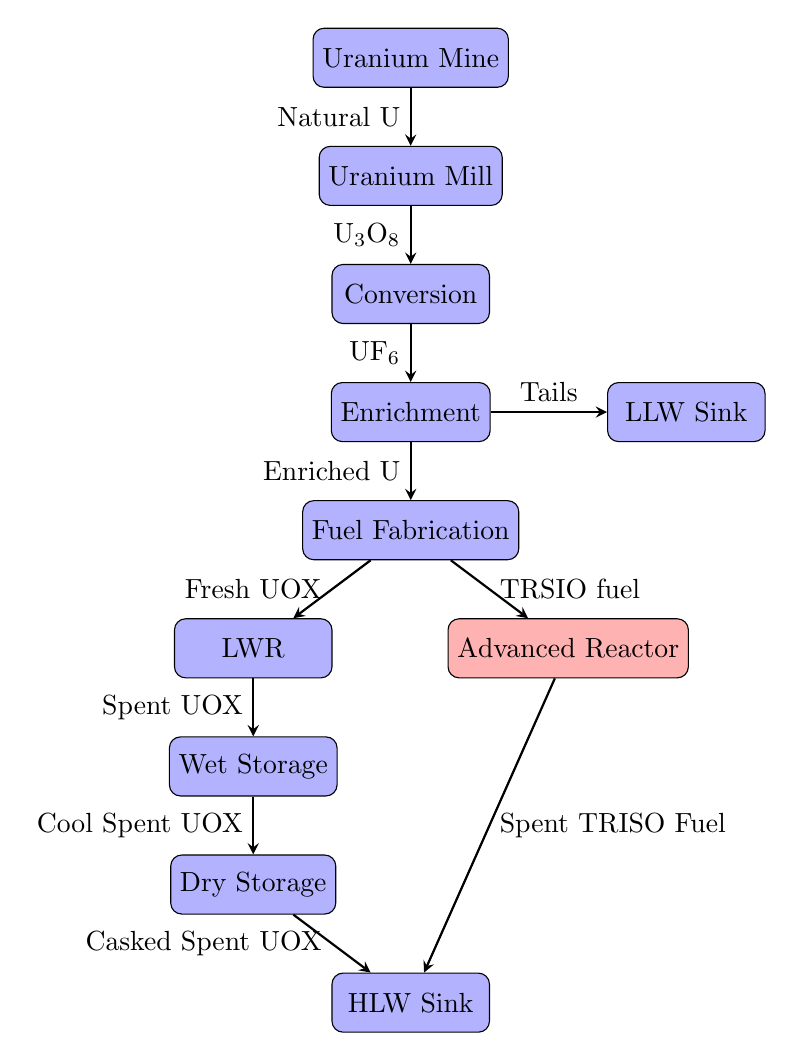
\begin{tikzpicture}[node distance=1.5cm]
            \node (mine) [facility] {Uranium Mine};
            \node (mill) [facility, below of=mine] {Uranium Mill};
            \node (conversion) [facility, below of=mill] {Conversion};
            \node (enrichment) [facility, below of=conversion]{Enrichment};
            \node (fabrication) [facility, below of=enrichment]{Fuel Fabrication};
            \node (reactor) [facility, below of=fabrication, xshift=-2cm]{LWR};
            \node (adv_reactor) [transition, below of=fabrication, xshift=2cm]{Advanced Reactor};
            \node (wetstorage) [facility, below of=reactor]{Wet Storage};
            \node (drystorage) [facility, below of=wetstorage]{Dry Storage};
            \node (sinkhlw) [facility, below of=drystorage, xshift=2cm]{HLW Sink};
            \node (sinkllw) [facility, right of=enrichment, xshift=2cm] {LLW Sink};
    
            \draw [arrow] (mine) -- node[anchor=east]{Natural U} (mill); 
            \draw [arrow] (mill) -- node[anchor=east]{U$_3$O$_8$}(conversion); 
            \draw [arrow] (conversion) -- node[anchor=east]{UF$_6$}(enrichment);
            \draw [arrow] (enrichment) -- node[anchor=east]{Enriched U}(fabrication);
            \draw [arrow] (enrichment) -- node[anchor=south]{Tails}(sinkllw);
            \draw [arrow] (fabrication) -- node[anchor=east]{Fresh UOX}(reactor);
            \draw [arrow] (fabrication) -- node[anchor=west]{TRSIO fuel}(adv_reactor);
            \draw [arrow] (reactor) -- node[anchor=east]{Spent UOX}(wetstorage);
            \draw [arrow] (wetstorage) -- node[anchor=east]{Cool Spent UOX}(drystorage);
            \draw [arrow] (drystorage) -- node[anchor=east]{Casked Spent UOX}(sinkhlw);
            \draw [arrow] (adv_reactor) -- node[anchor=west]{Spent TRISO Fuel}(sinkhlw);
    
            \end{tikzpicture}
        \caption{Fuel cycle facilities and material flow between facilities. Facilities in 
        red are deployed in the transition scenarios.}
        \label{fig:fuel_cycle}
    \end{figure}

The composition of the materials shown in Figure \ref{fig:fuel_cycle} 
are defined using recipes. Spent and fresh \gls{LWR} 
fuel recipes were obtained from \cite{yacout_visionverifiable_2006}. 
The spent \gls{LWR} fuel 
recipe assumes a 51 MWd/kg-U burnup. All other recipes capture the 
necessary isotopic ratios of uranium, but do not include other elements.
Neutronic or depletion simualtions were not modeled as part of this work.  
The enrichment feed recipe assumes natural uranium is used, and the tails 
assay is 0.2\%. 
\section{Results}

This is the results section.

\begin{align}
	F &= ma \\
	\intertext{where:}
	F &= \text{net force applied on the body [N]} \nonumber \\
	m &= \text{total mass of the body [kg]} \nonumber \\
	a &= \text{net acceleration of the body [m s}^{-2}\text{]} \nonumber
\end{align}

\begin{figure}[htbp!]
	\begin{center}
		
\includegraphics[scale=0.7]{./images/catinhat}
	\end{center}
	\caption{A caption for the figure.}
	\label{fig:catinhat}
\end{figure}

\begin{table}[h]
	\centering
        \caption{A caption for the table.}
\begin{tabular}{lr}
	\hline
	\textbf{Properties} & \textbf{Value} \\
	\hline
    Mass [kg] & 2,324 \\
    Height [m] & 558 \\
    Volume [m$^3$] & 4,072 \\
    \hline
\end{tabular}
\label{tab:table1}
\end {table}

\section{Conclusions}
This work simulated multiple fuel cycle scenarios to compare the 
material requirements of deploying different advanced reactors fueled 
by \gls{HALEU}. Scenarios include a no-growth and a 1\% growth 
transitions to either the \gls{USNC} \gls{MMR} or the X-energy Xe-100 
reactor from the current fleet of U.S. \glspl{LWR}. We used the current 
fleet of \glspl{LWR}, without a transition to an advanced reactor for 
comparison. Each of these scenarios are compared for their material 
requirements, specifically the number of reactors deployed, the mass 
of enriched uranium sent to the reactors, and the \gls{SWU} capacity 
required to enrich natural uranium to produce the fuel needed for 
each scenario. 

More \glspl{MMR} are required than Xe-100 reactors to meet the same 
energy demand, because of the differences in their power output. 
The transition scenarios exhibit some gaps between  
energy production and demand, localized to the beginning of the 
transition
scenarios, and to the replacement of \glspl{MMR} as they are decommissioned. 
Xe-100 reactors are not decommissioned in the simulated time frame because 
their lifetime exceeds the time span simulated. Therefore, the 
energy produced and the material requirements for the replacement of 
Xe-100 reactors is not explored in this work. 

Transitioning to the \gls{MMR} requires 
a larger average mass and \gls{SWU} capacity than transitioning to the 
Xe-100 reactors. Transitioning to the \gls{MMR} requires a smaller average 
uranium mass but a greater \gls{SWU} capacity than fueling \glspl{LWR} prior 
to 2025 because the \gls{MMR} requires a higher enrichment level. 
Fueling \glspl{MMR} involves large, one-time shipments of fuel, while 
fueling the Xe-100 involves small, continuous shipments of fuel 
because of the different refueling schemes.

\section{Future Work}
One possible area of future work is extending the end date 
of the scenarios to 2125 to investigate how replacing deployed Xe-100 
reactors impacts the material requirements and energy produced in those 
transition scenarios. Another area of future work is to investigate the 
material requirements if the \gls{HALEU} demand is met by downblending 
\gls{HEU} or enriching uranium of non-natural enrichment, such as 
\gls{LEU} below 5\% $^{235}$U. Finally, an investigation into the 
optimization of an enrichment facility or the use of other methods to 
create \gls{HALEU} to meet the demand of each scenario will provide 
insight into the logistics of transitioning to \gls{HALEU}-fueled 
reactors. 

\section{Acknowledgments}
This material is based upon work supported under an Integrated University Program Graduate
Fellowship.

The authors would like to thank Nathan Ryan of the University of Illinois 
Urbana-Champaign for his assistance in technical editing.

\bibliography{bibliography}

% Prof. Huff discourages appendices in journal articles.
% But, if you must, include one like so:
%\pagebreak
%
\appendix
\section{}


\end{document}
